\section*{Question 3}
\subsection*{(a)}
The resulting decision boundary is a linear combination of the decision boundaries of the weak learners.

\subsection*{(b)}
$p$ is also a very important parameter of this classifier. We had to extend everything (also in the following subtasks) to include $p$.

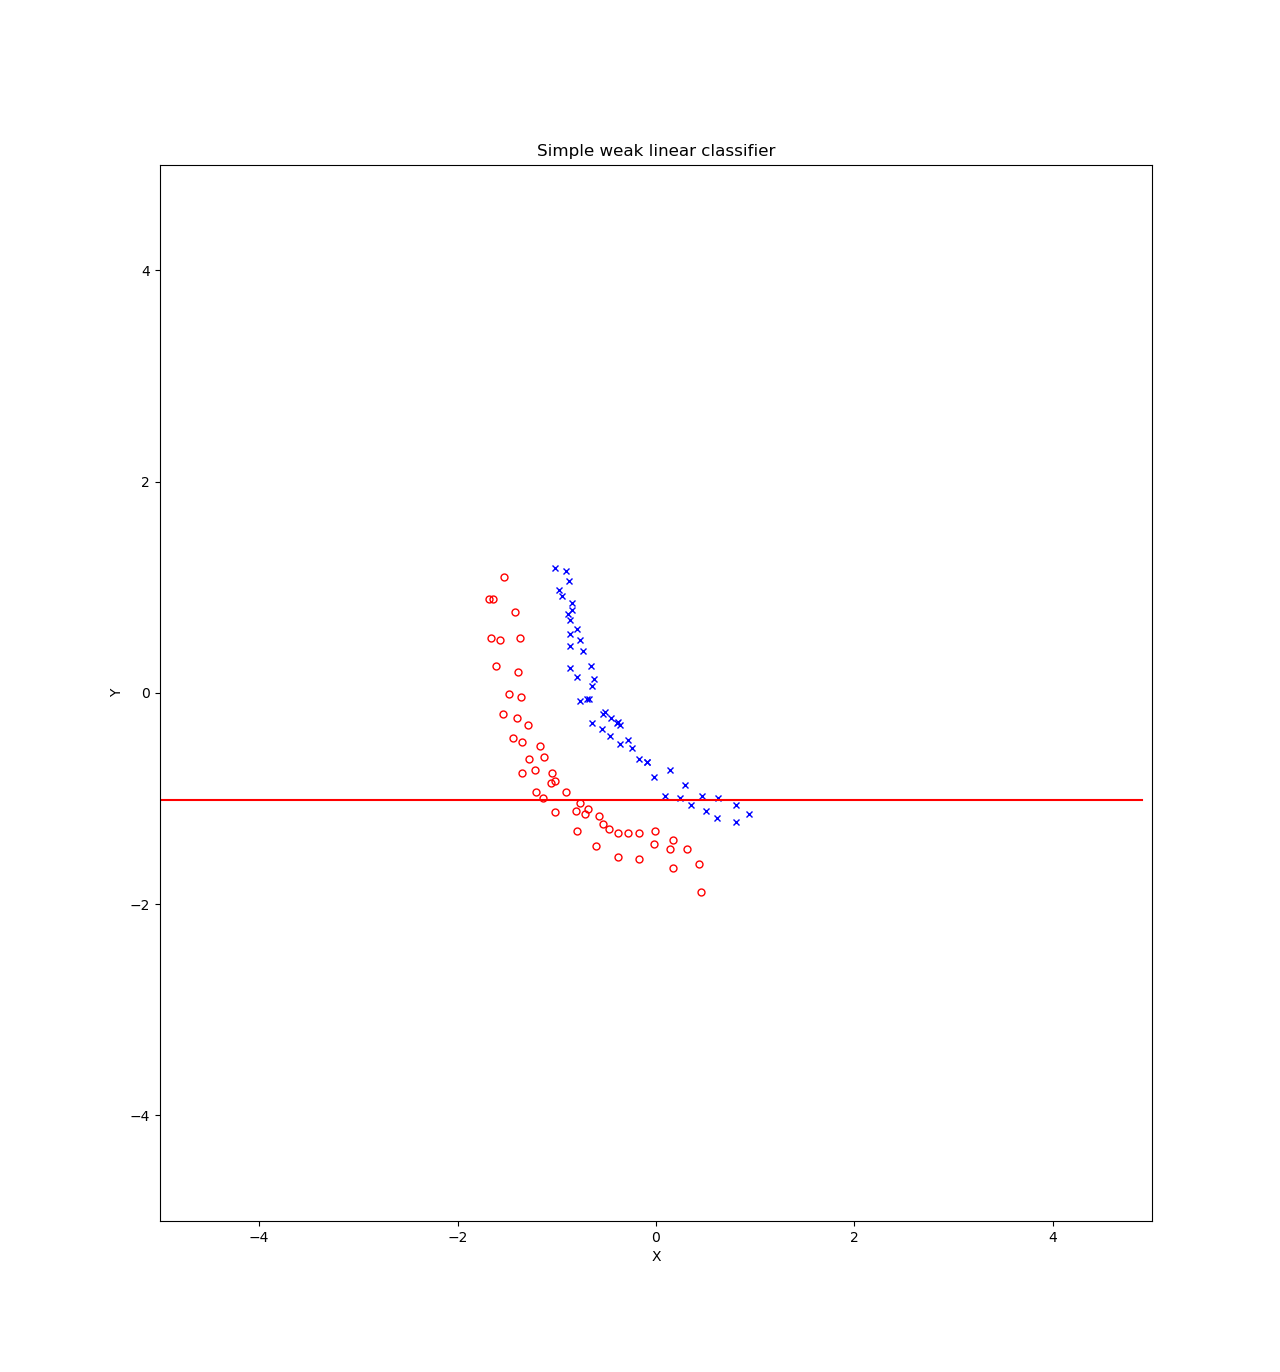
\includegraphics[width=.5\textwidth]{q3_adaboost_python/Figure_WEAK.png}

\subsection*{(c)}
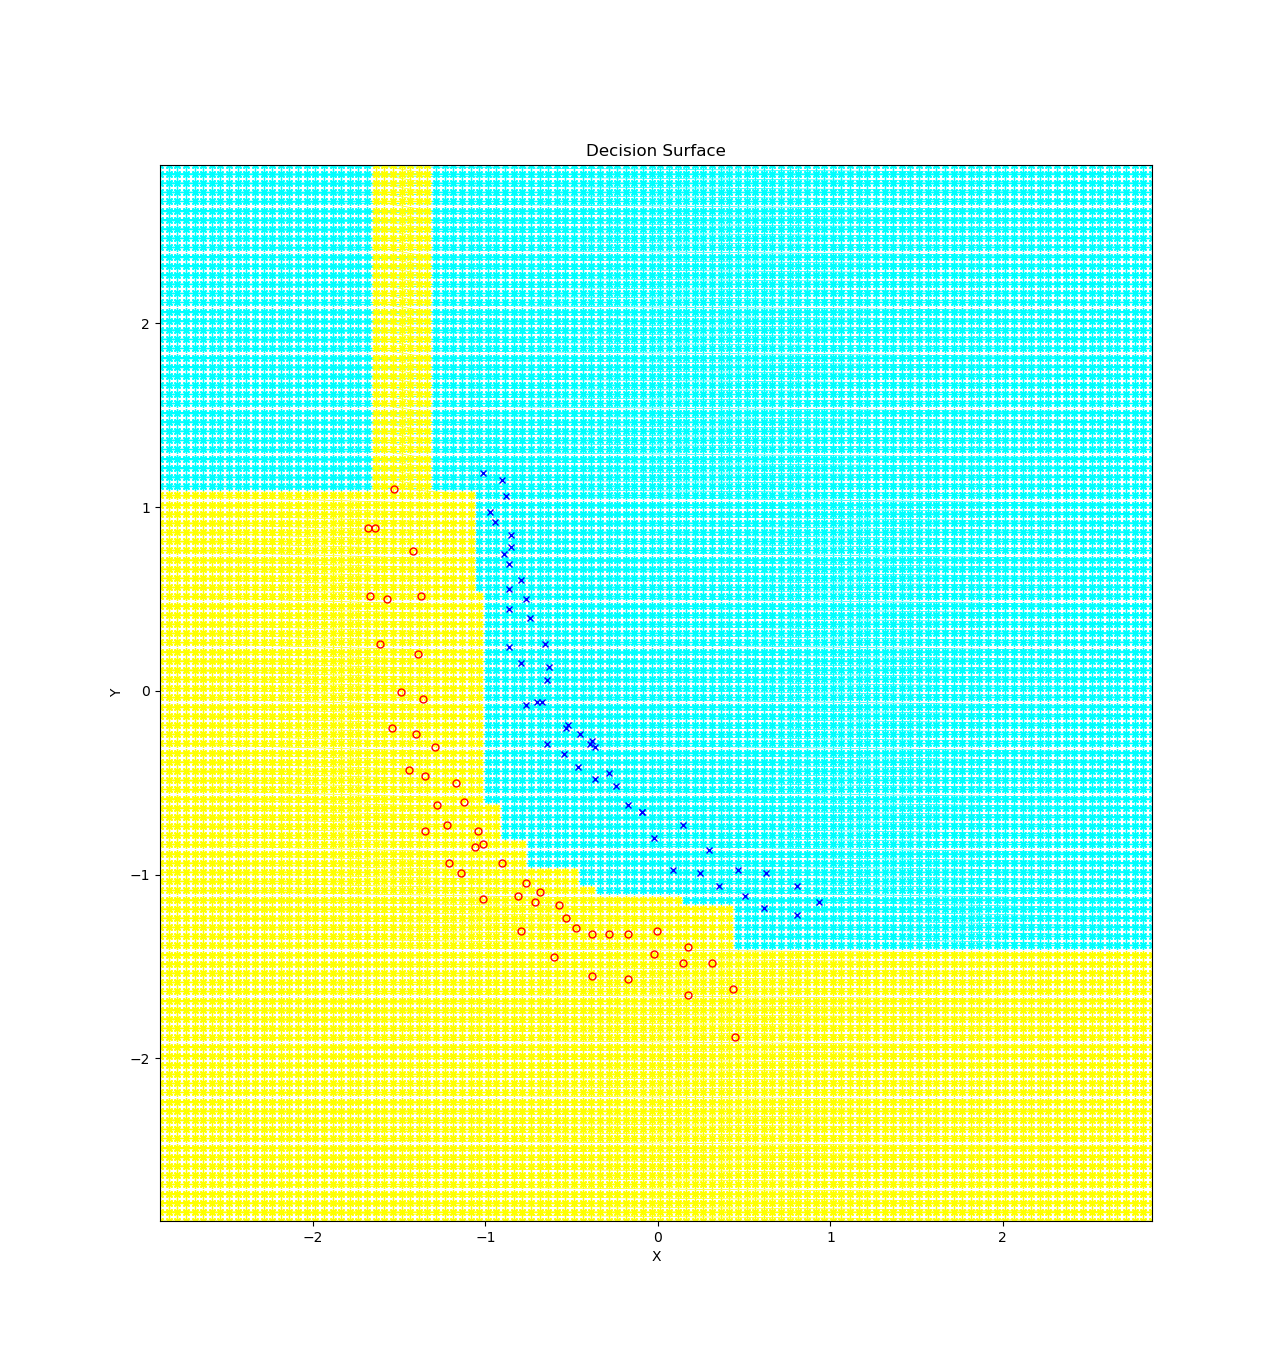
\includegraphics[width=.5\textwidth]{q3_adaboost_python/Figure_ADA_SIMPLE_1.png}
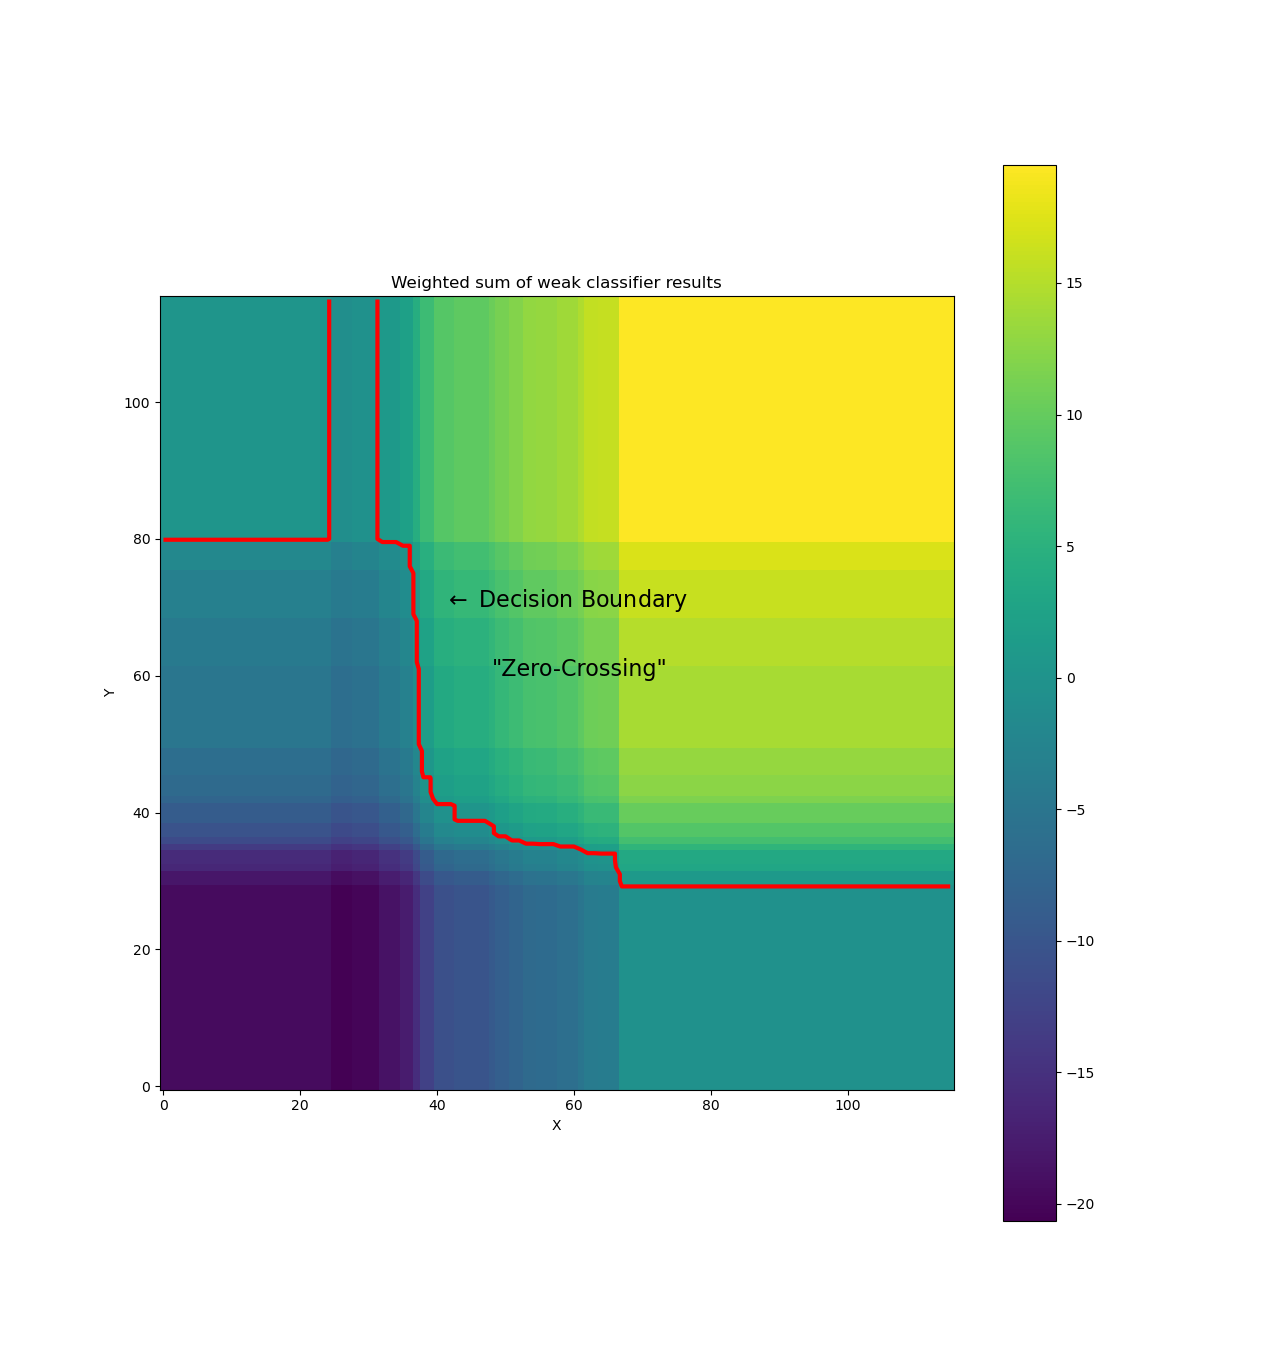
\includegraphics[width=.5\textwidth]{q3_adaboost_python/Figure_ADA_SIMPLE_2.png}

\subsection*{(d)}
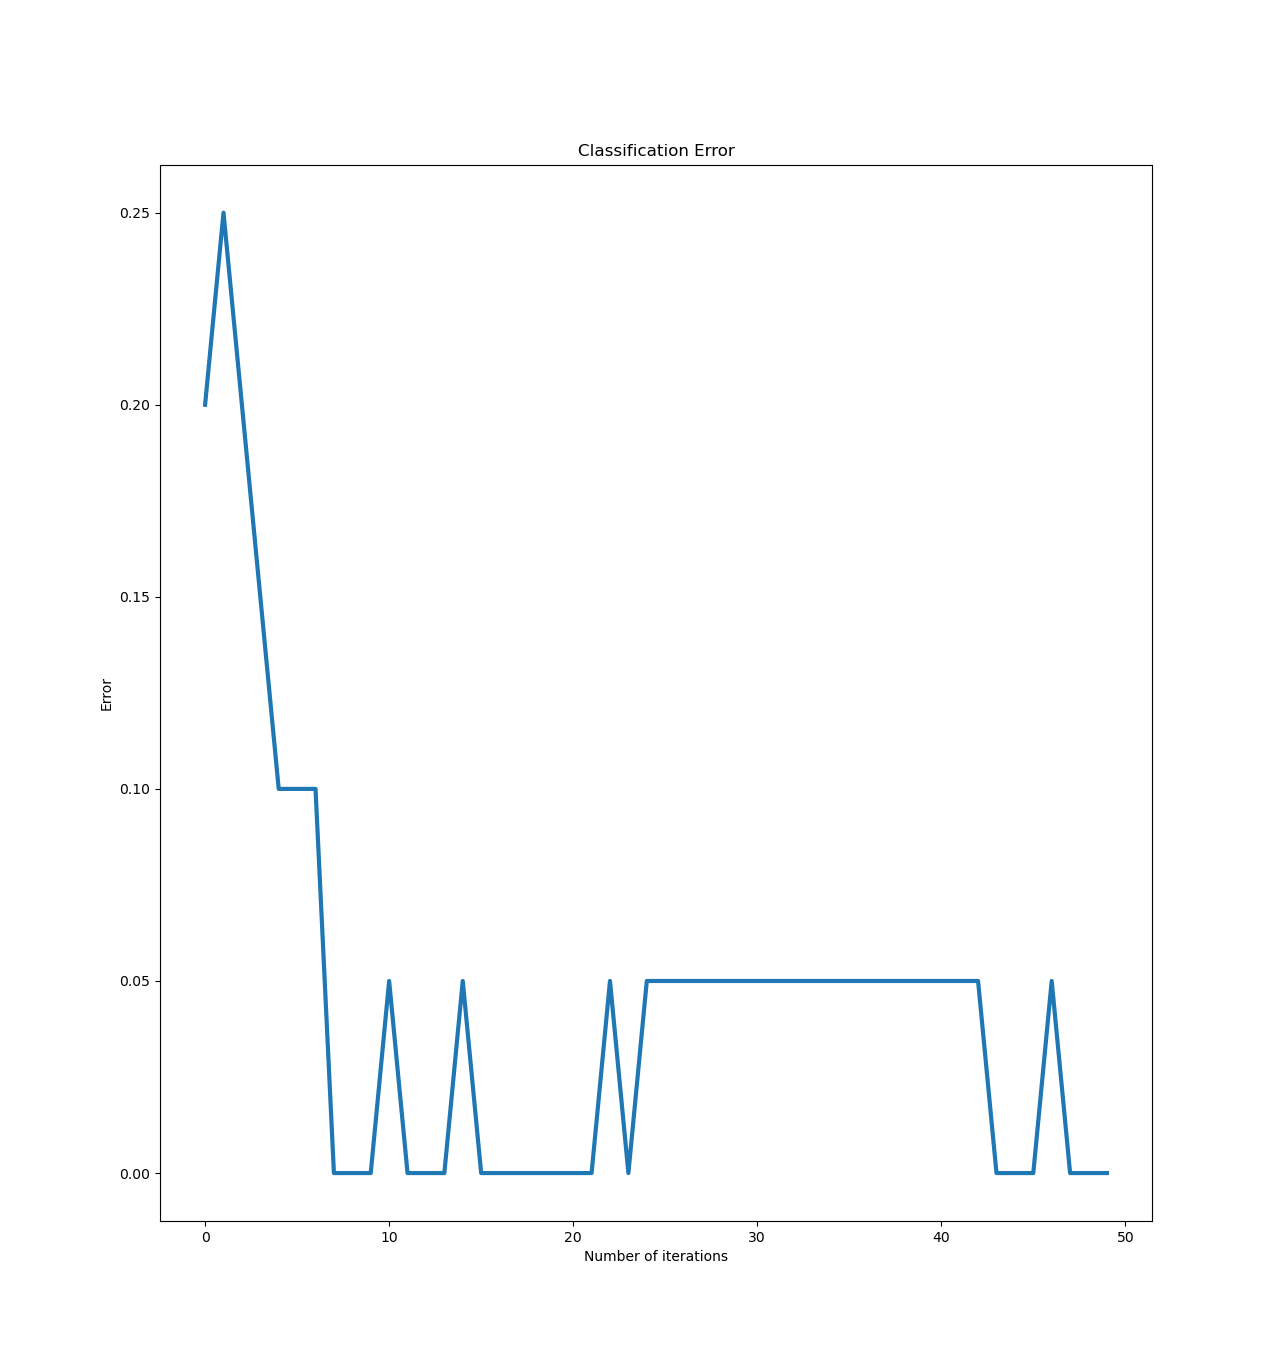
\includegraphics[width=.5\textwidth]{q3_adaboost_python/Figure_CROSS_1.png}
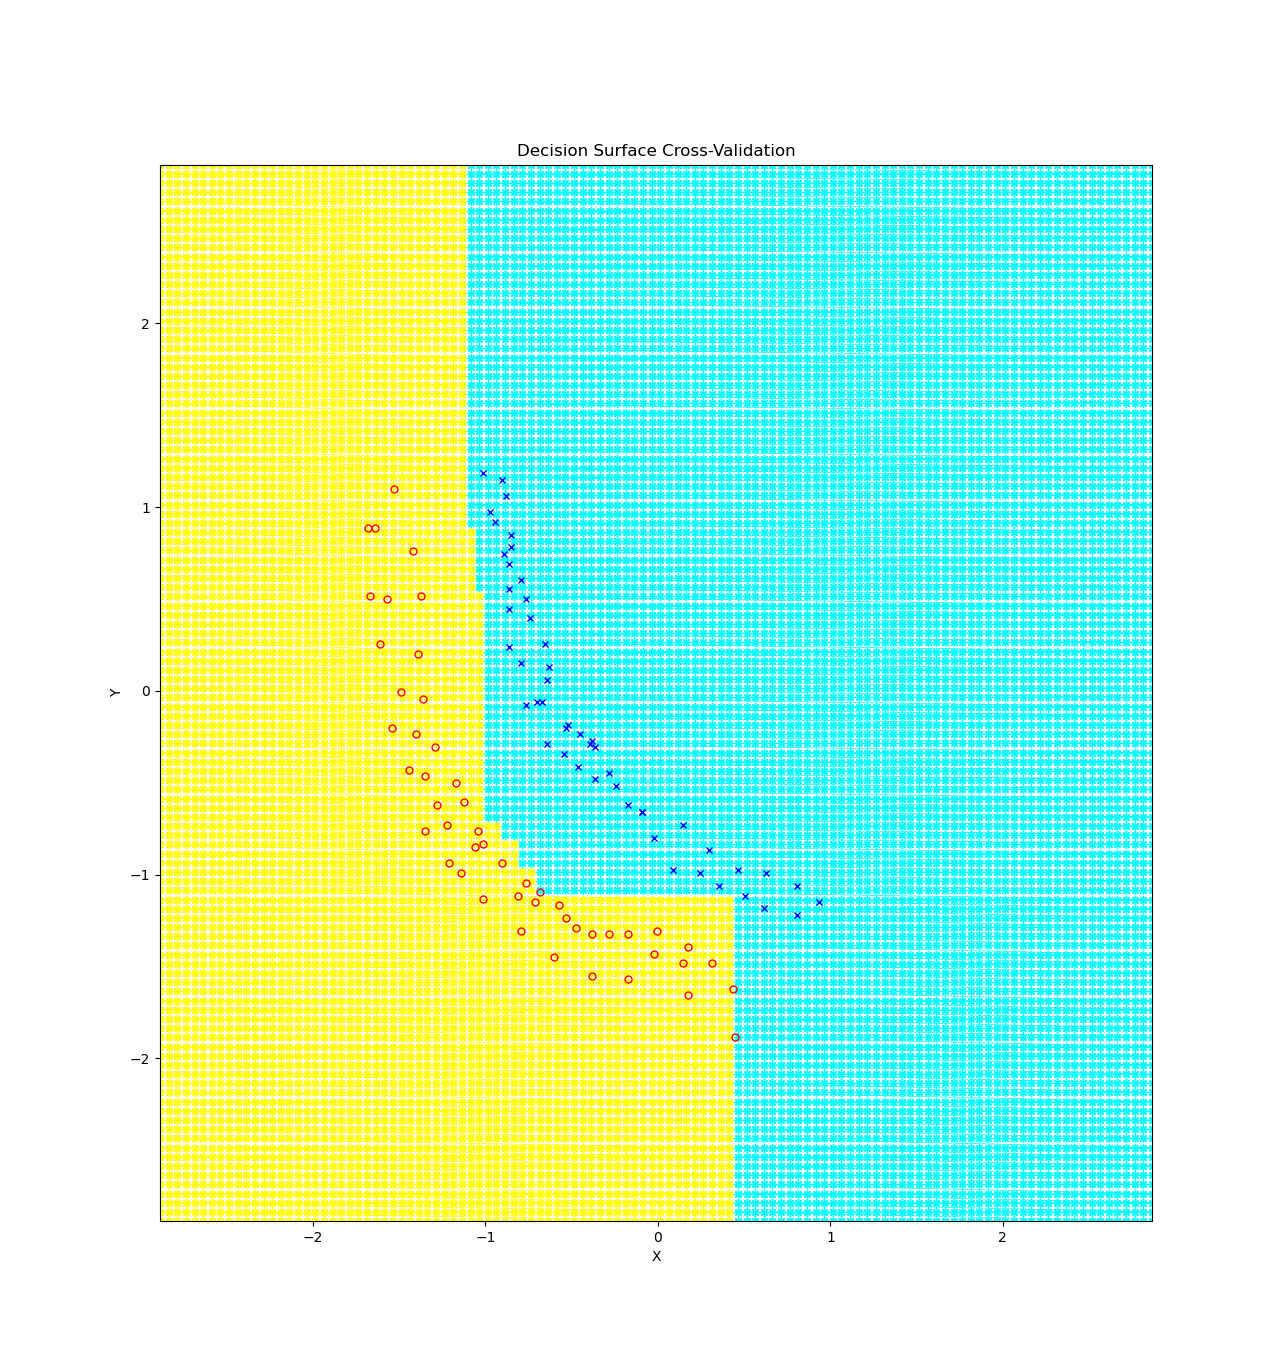
\includegraphics[width=.5\textwidth]{q3_adaboost_python/Figure_CROSS_2.png}
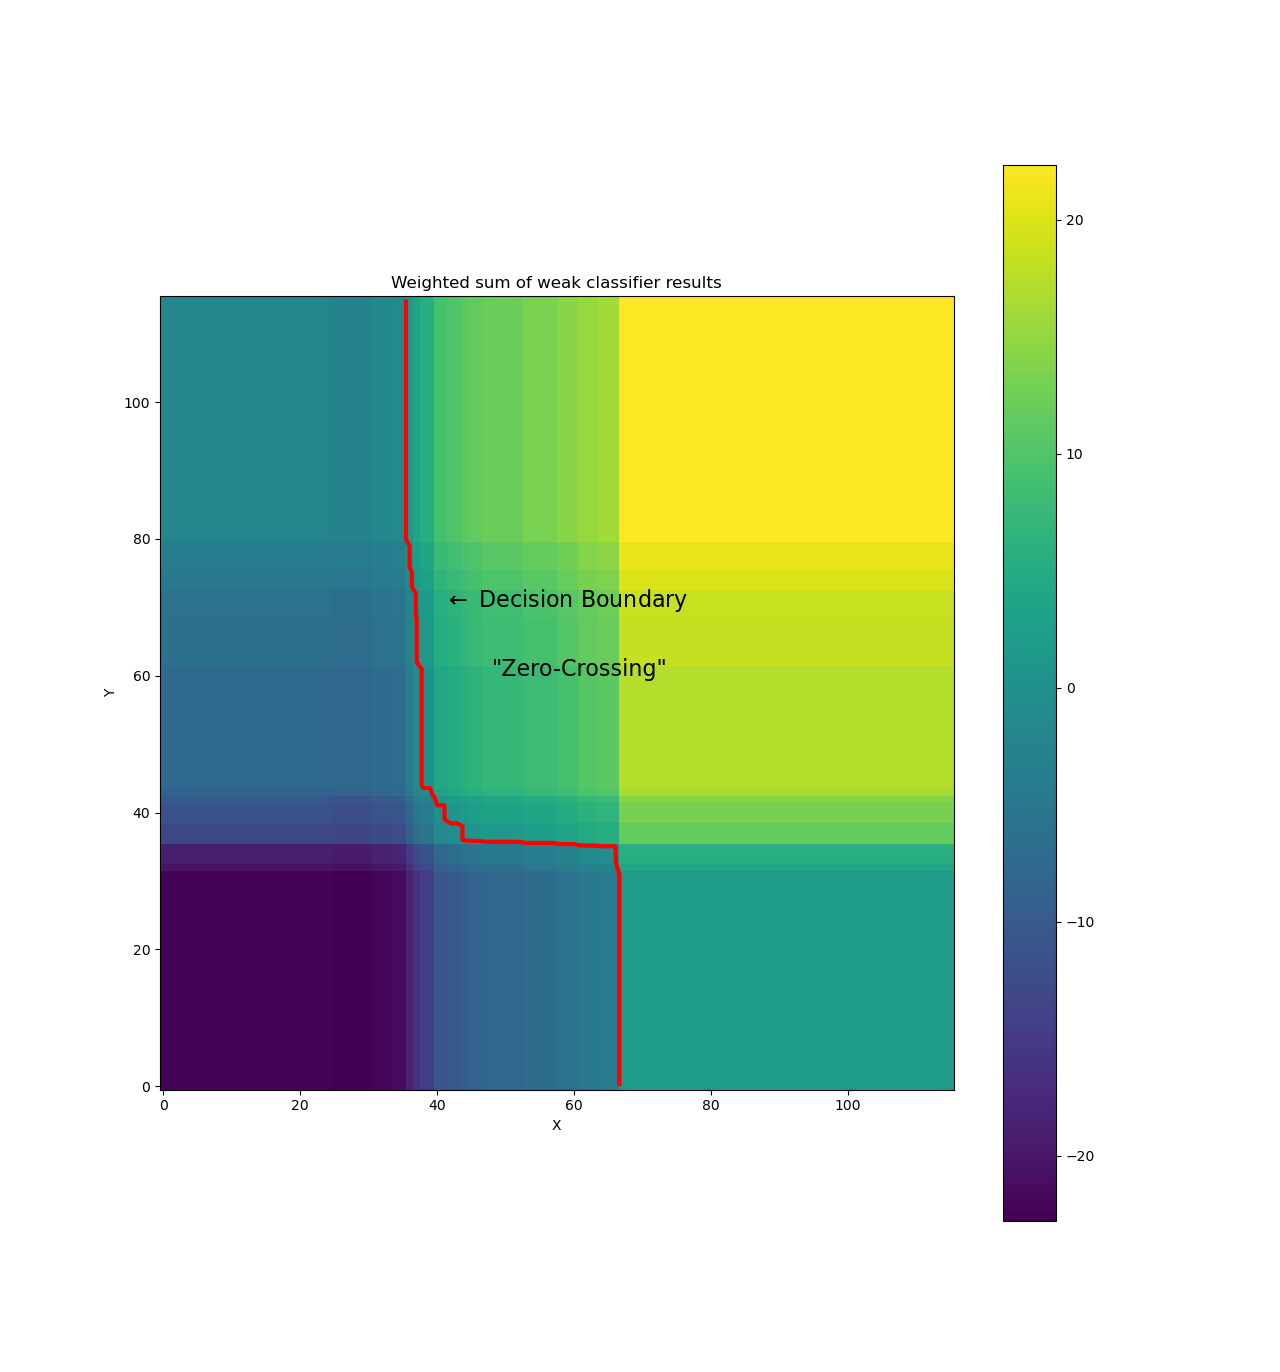
\includegraphics[width=.5\textwidth]{q3_adaboost_python/Figure_CROSS_3.png}

\subsection*{(e)}
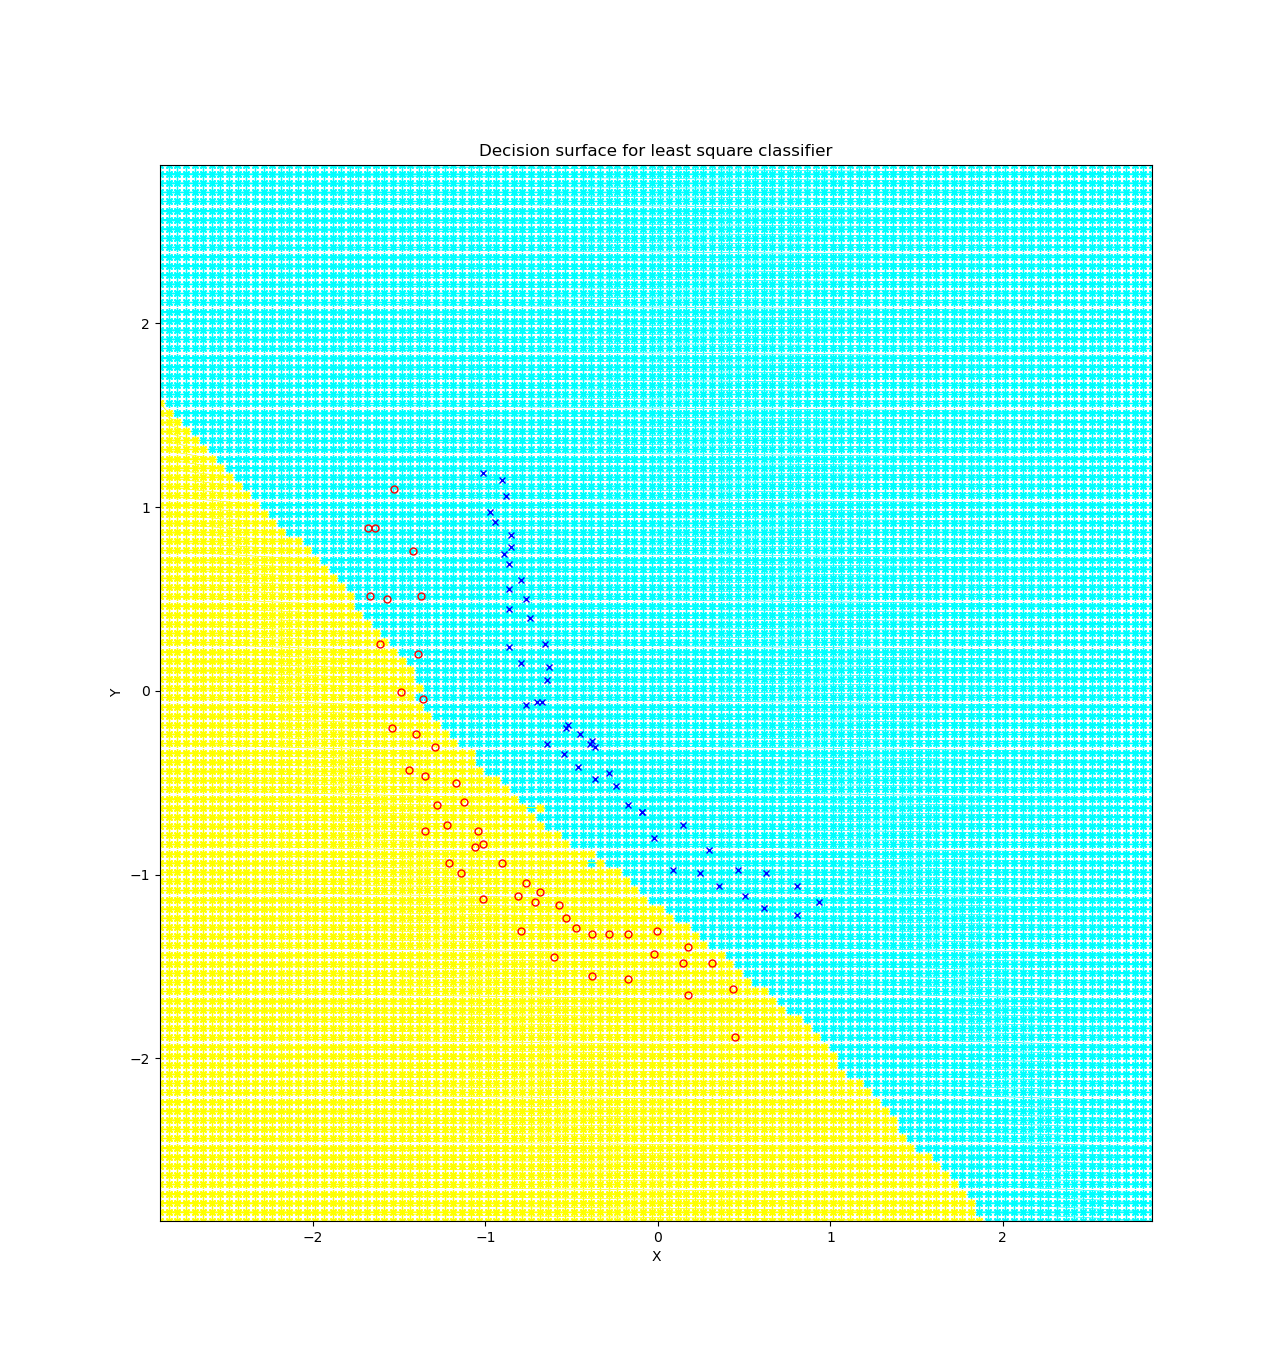
\includegraphics[width=.5\textwidth]{q3_adaboost_python/Figure_ADA_LSLC_1.png}
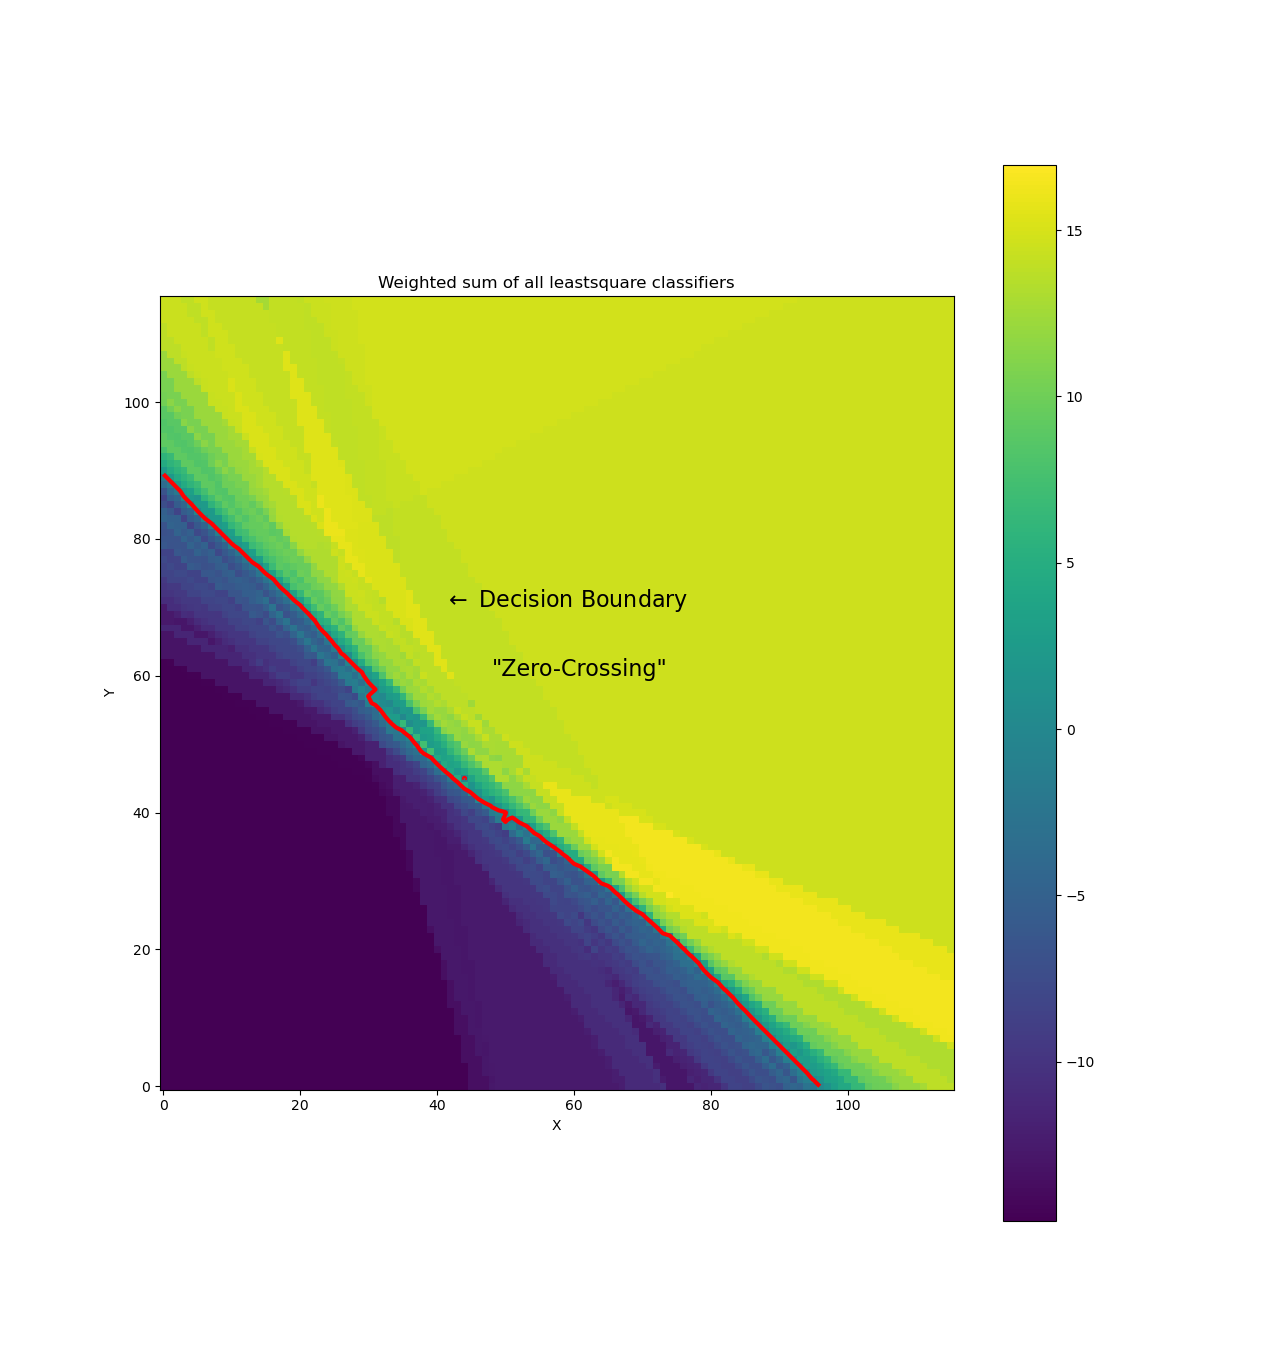
\includegraphics[width=.5\textwidth]{q3_adaboost_python/Figure_ADA_LSLC_2.png}
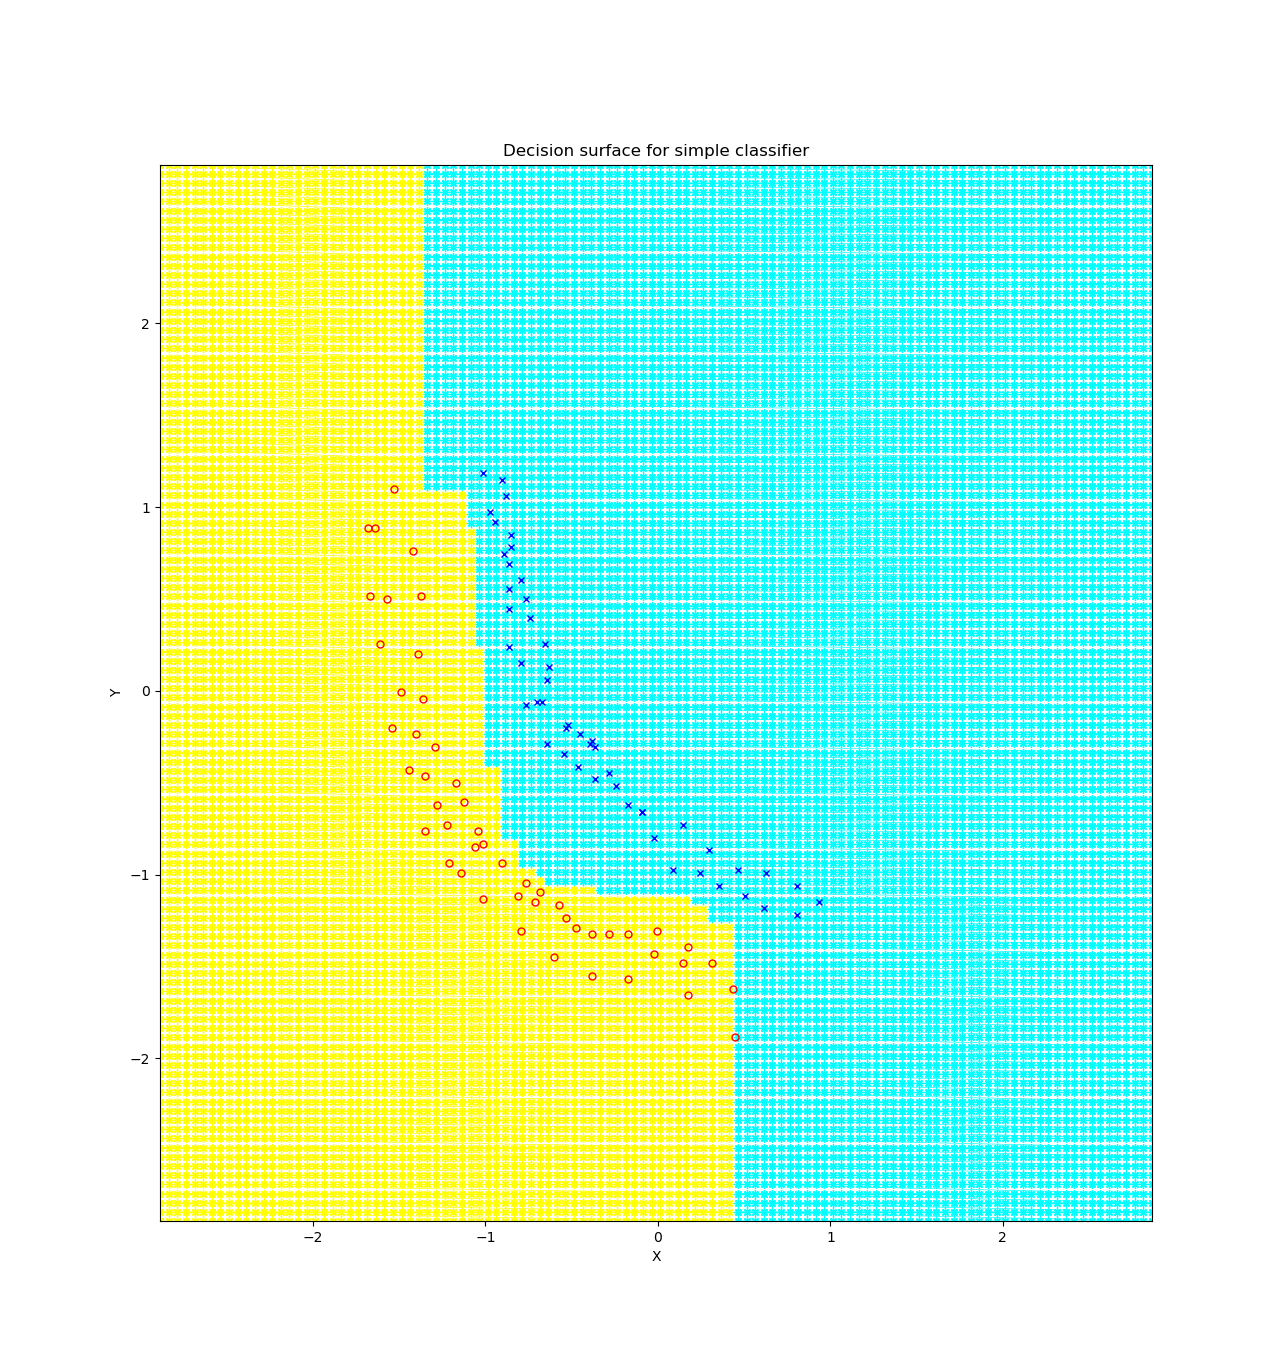
\includegraphics[width=.5\textwidth]{q3_adaboost_python/Figure_ADA_LSLC_3.png}
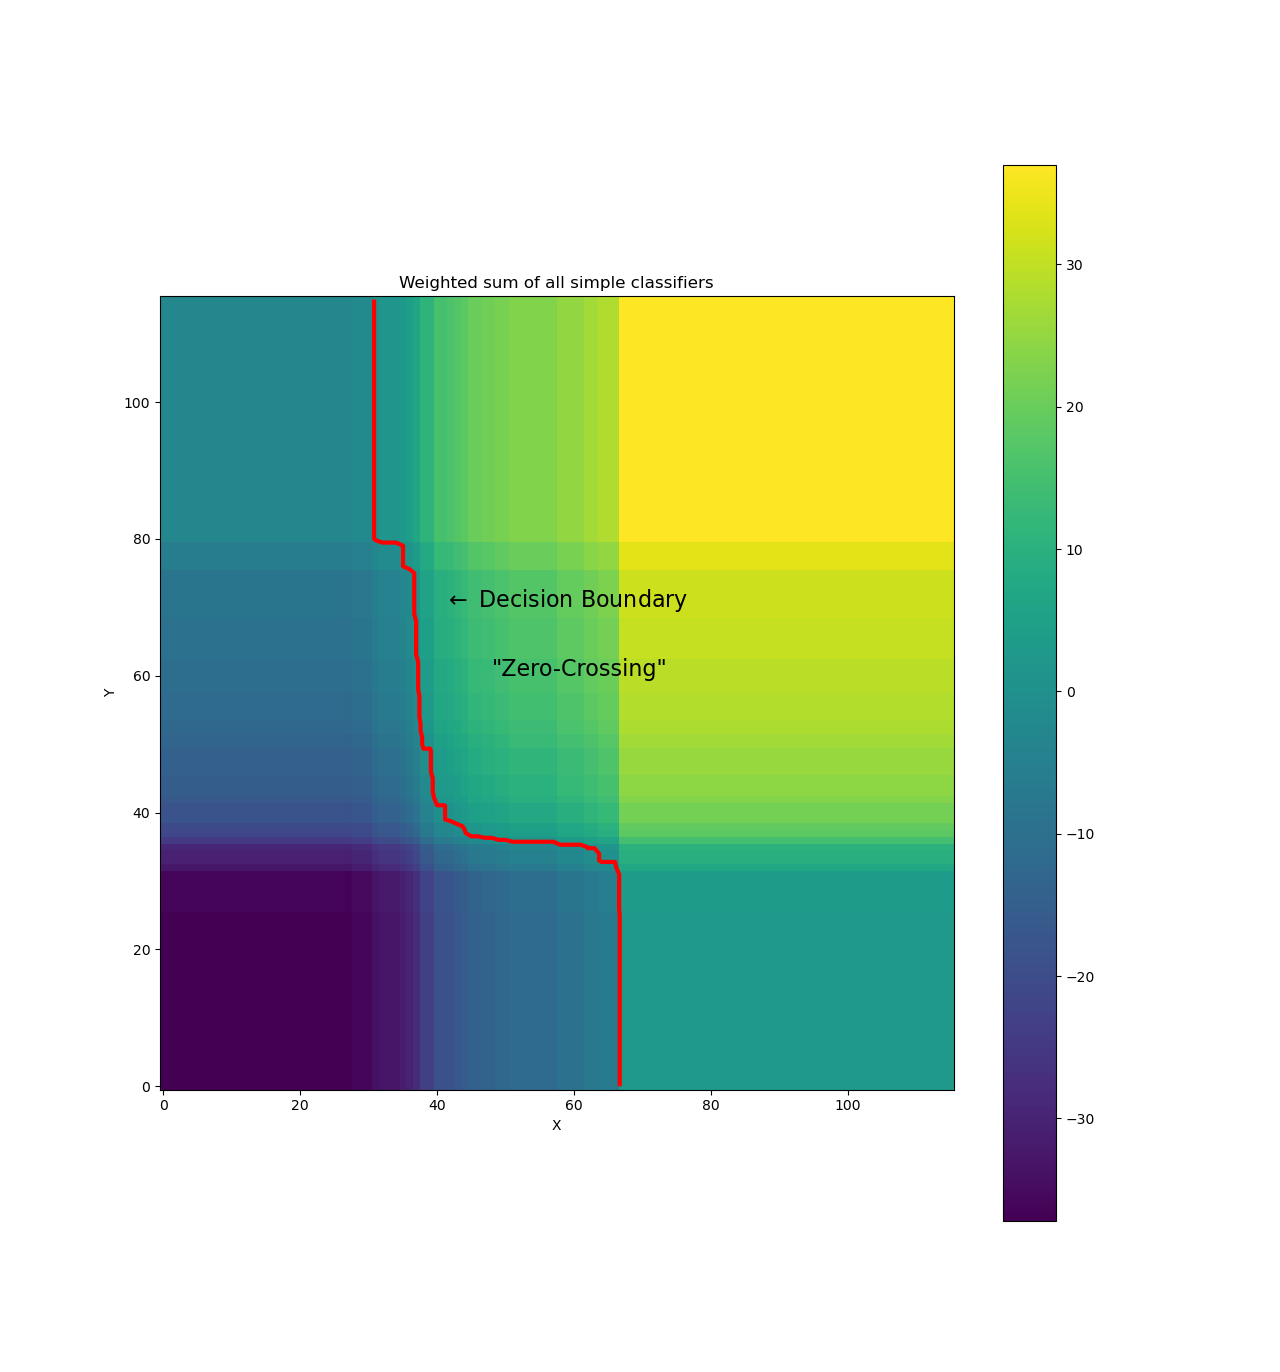
\includegraphics[width=.5\textwidth]{q3_adaboost_python/Figure_ADA_LSLC_4.png}

\subsection*{(f)}
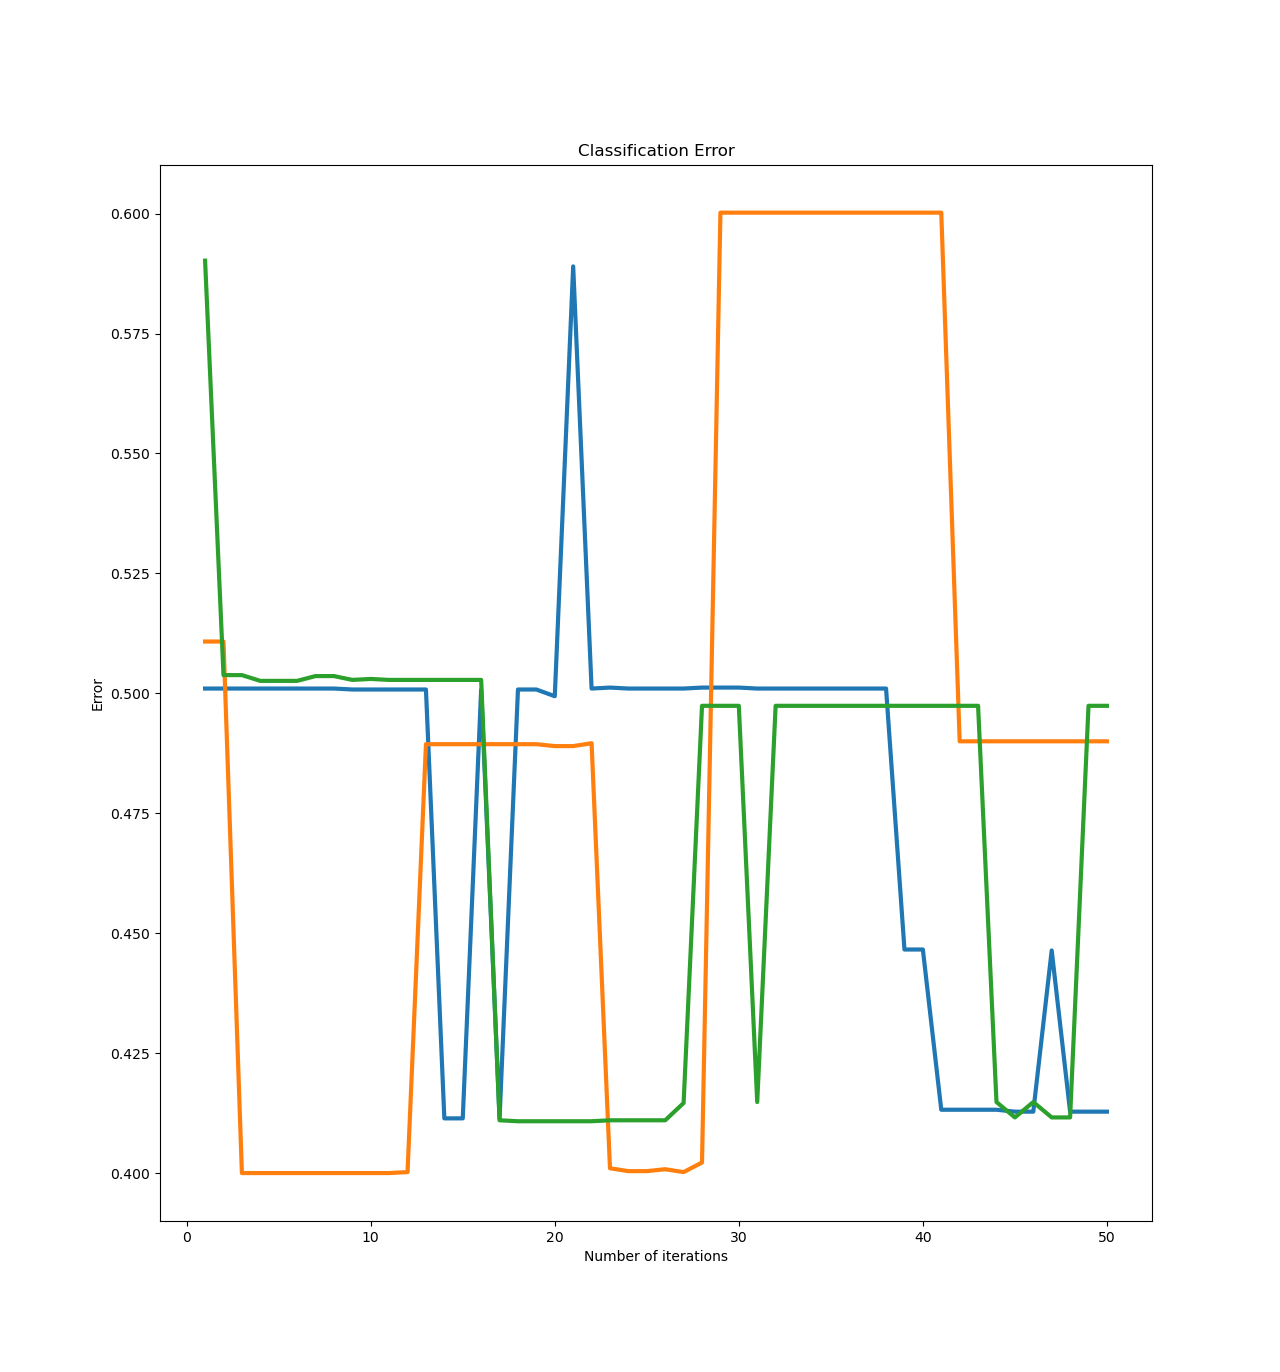
\includegraphics[width=.5\textwidth]{q3_adaboost_python/Figure_USPS_1.png}
